\section{Introduction and motivation}
\label{sec:Introduction}

This is the reference~\cite{Gligorov:2017nwh}
\newline
\textbf{``The results shown are unofficial and have not been formally approved by the LHCb collaboration"}

\subsection{Motivations}

There is no clear observation of new physics (NP) at the LHC as yet. The NP portal is considered in weakly coupled sector with long lifetime. 
The long lifetimes are very generic in any theory with multiple mass scales, broken symmetries and so on. 
Standard Model (SM) is a good example since it contains low mass particles with long lifetime such as electron, neutrino, proton and neutron.
%There are several experiments for searching LLPs. MATHUSLA (\atlas), MilliQan (\cms), SHiP. 
%But these experiments are so large to compare with CODEX-b, this is a one attractive of CODEX-b. 
%We can control backgrounds because it will be placed underground and shields are existed. 

\subsection{Compact Detector for Exotics at LHCb}

The Compact Detector for Exotics at \lhcb (CODEX-b) was proposed to observe weakly coupled \textbf{LLP}s in \lhcb cavern. 
Since \atlas and \cms focused on high \pt and large QCD backgrounds and restricted lifetime of \lhcb, current detectors can miss signals from weakly coupled \textbf{LLP}s. 
By following the fig.~1, the DAQ racks will be moved to the surface before run~3 and the CODEX-b will be placed at the site with 10 X 10 X 10~m size. 
The CODEX-b aparts 25~m from the impact point~8. 
If the \delphi is removed, the size can be expanded to 20 X 10 X 10~m.
%The CODEX-b consists of two parts. 
%6 RPC layers at 4\cm intervals on each box face with 1\cm granularity (Attach the geometry plot of CODEX-b here!!). 
%5 equally spaced triplets along the depth to minimize distance between reconstructed vertex and 1st measurement. 
%50 - 100 ps timing from RPC's foreseenfor mass reconstruction.
%Additional passive Pb shield to suppress muon and neutral hadrons. 
%Thin active veto for secondaries inside the shield. 

\begin{figure}[h]
\centering
    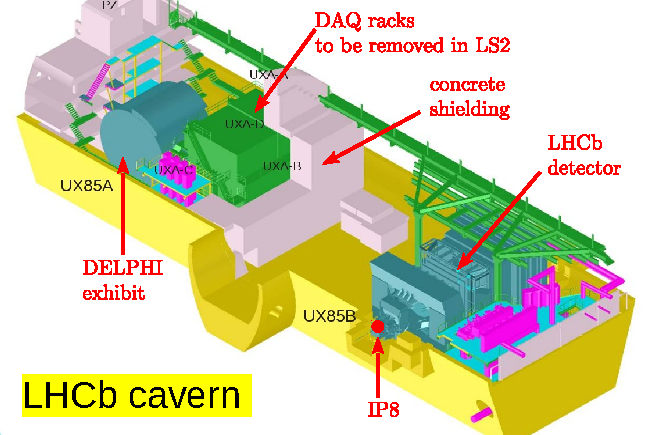
\includegraphics[width=12cm]{figs/INT/lhcb_cavern.pdf}
    \vspace{0.15cm}
\caption{ 
   Schematic plot of LHCb cavern 
}
\end{figure}
